\documentclass[10pt]{article}

%%%%%%%%%%%%%%%%%%%%%%%%%
% Package configuration %
%%%%%%%%%%%%%%%%%%%%%%%%%

% Page margin
\usepackage[margin=1in]{geometry}

% Support for bold small cap font
\usepackage[tuenc]{fontspec}
\setmainfont[
    Path=./fonts/,
    Extension=.otf,
    BoldFont=cmu-serif-bold,
    BoldItalicFont=cmu-serif-bold-italic,
    ItalicFont=cmu-serif-italic,
]{cmu-serif}

% Better typesetting quality
\usepackage{microtype}

% Math
\usepackage{amsmath}

% SI-units
\usepackage{siunitx}

% Redefine section, subsection styles
\usepackage[compact,center,explicit]{titlesec}
\usepackage{textcase}
\titleformat{\section}{\scshape\lsstyle\normalsize\filcenter}
    {\thesection}{1em}{\MakeTextUppercase{#1}}
\titleformat{\subsection}{\normalfont\small\bfseries\filcenter}
    {\thesubsection}{1em}{#1}

% PRL-style horizontal rule
\usepackage{graphicx,amssymb}
\newcommand{\PRLrule}{
    \bigskip
    \noindent\makebox[\linewidth]{
        \resizebox{0.3333\linewidth}{1pt}{$\blacklozenge$}
    }
    \bigskip
}

% Bold math in section title
\makeatletter
\g@addto@macro\bfseries{\boldmath}
\makeatother

% Set up link
\usepackage{hyperref}
\hypersetup{colorlinks,breaklinks,citecolor=blue}

% Set up author affiliation
\usepackage[affil-it]{authblk}

% Set up biblatex database
\usepackage[
    %style=phys,
    giveninits=true,
    %backref=true,
    natbib=true,
    backend=biber,
    doi=true,
    % Sort by the order of citation
    sorting=none,
    % This options ensures that no automatic et al. is generated
    %maxbibnames=99,
    % This option must be enabled with 'babel' package
    useprefix=false
]{biblatex}
\addbibresource{umd_phd_candidacy_paper.bib}


%%%%%%%%%%%%%%%%%
% User settings %
%%%%%%%%%%%%%%%%%

% User-defined variables
\def\BaBar/{\textsc{BaBar}}
\def\Y4S/{\ensuremath{\Upsilon(\text{4S})}}

% Title info
\title{Review on Testing lepton flavor universality in semileptonic channels}
\author{Yipeng Sun}
\affil{Department of Physics, University of Maryland}
\date{\today}


%%%%%%%%%%%
% Content %
%%%%%%%%%%%

\begin{document}
\maketitle

\begin{abstract}
    What is LFUV? (FU physics, FUV physics)
    Why semileptonic decays (good thing about form factor)?
    A historical review, starting from 2012 BaBar;
    Talk about Phoebe's run 1 analyses.
    Talk about what we are doing.
    Talk about expected improvements and drawbacks of our upcoming analysis compared
    to run 1.
\end{abstract}

\section{Theory}
% Lepton flavor universality (LFU) and LFU violation (LFUV)
% vim: ft=tex:

\subsection{Lepton flavor universality}
The standard model (SM) Lagrangian manifests that all three flavors of leptons
have exactly the same coupling to all SM processes\footnote{
    I'll talk about Higgs mechanism in a later section.
}.


\subsection{Advantages of semileptonic channel decays}

\subsection{Higgs mechanism}

\subsection{2-Higgs doublet models (2HDM)}
% type-II model claimed to be excluded; type-III (very similar to type-II) still
% alive.

\subsection{Leptoquark models}


\section{Review for detectors/colliders used in testing LFU}
The LFU has been tested in many precision measurements.
The majority of them involve the difference between the decay rates of $B$
mesons to $\tau$ and $\mu$.

% Why not J/psi (c cbar, mass ~ 3.10 GeV, mass of tau ~ 1.77 GeV)?
One may ask: Why are we so focused on $b$ quark bound states and mesons?
After all, $J/\psi$, a $c\bar{c}$ bound state, is already kinematically allowed
to decay into all three generations of leptons.
The main reason is:
% Initially B factories are meant for CP violation detection.
Initially, detectors of $B$ factories, such as \BaBar/ at PEP-II, were
primarily constructed to for precision measurements on CP violation of $B^0$,
for SM predicts ``large, calculable'' CP violation in the decay of these mesons
\cite{Luth:1994}.
But these detectors proved to be advantageous in the testing of LFU:
These measurements have very similar requirements on the
detector \cite{Boutigny:1995ib}.
Thus, testing of LFU is often part of the secondary goals of these
experiments \cite{Luth:1994}.

In this section, I will review \BaBar/ detector at the PEP-II collider, and LHCb
at the Large Hadron Collider (LHC)---both have conducted various tests on LFU.
These detectors/colliders are representative of the detectors for
electron-position colliders and hadron colliders.

% Talk about PEP-II and its asymmetrical beam energies
PEP-II is an asymmetrical $e^- e^+$ collider at SLAC.
In PEP-II, $B$ mesons are produced primarily in the following process:
$e^- e^+ \rightarrow \Y4S/ \rightarrow B \bar{B}$, with
$e^-$ and $e^+$ beams tuned at different energies,
such that the invariant mass is at the \Y4S/ resonance (\SI{10.58}{GeV}),
and the momentum of the \Y4S/ in the lab frame
non-zero \cite{Harrison:1998yr}.

Producing at \Y4S/ peak eliminates almost all fragmentation products, reducing
combinatorial background.
Also, since the momenta of $e^- e^+$ is known, with the reconstruction of the
momentum of one $B$ meson ($B_{tag}$), the rest frame of the other $B$
($B_{sig}$) can be calculated as
\begin{equation}
    p_{B_{sig}} = p_{e^-e^+} - p_{B_{tag}}.
\end{equation}
Later we will see that this makes identifying events that have more than one
missing particle easier.

% Talk about subdetectors
\BaBar/ is a barrel detector (shown in \autoref{fig:babar_detector_view})
that consists of five subdetectors.
From inside out:
Silicon Vertex Tracker (SVT) and Drift Chamber (DCH), which measure the momenta
and angles of charged particles.
Detector of Internally Reflected Cerenkov radiation (DIRC), together with SVT
and DCH, identifies charged particles of different masses by Cerenkov
ring-imaging and ionization energy loss of these particles.
Caesium Iodide Electromagnetic Calorimeter (EMC), which measures energy and
position of electromagnetic showers generated by electrons and photons.
A superconducting solenoid with a \SI{1.5}{T} magnetic field surrounding the
EMC, together with Instrumented Flux Return (IFR), is used to identify muons and
some neutral hadrons \cite{Lees:2013uzd}.

\begin{figure}[ht]
    \centering
    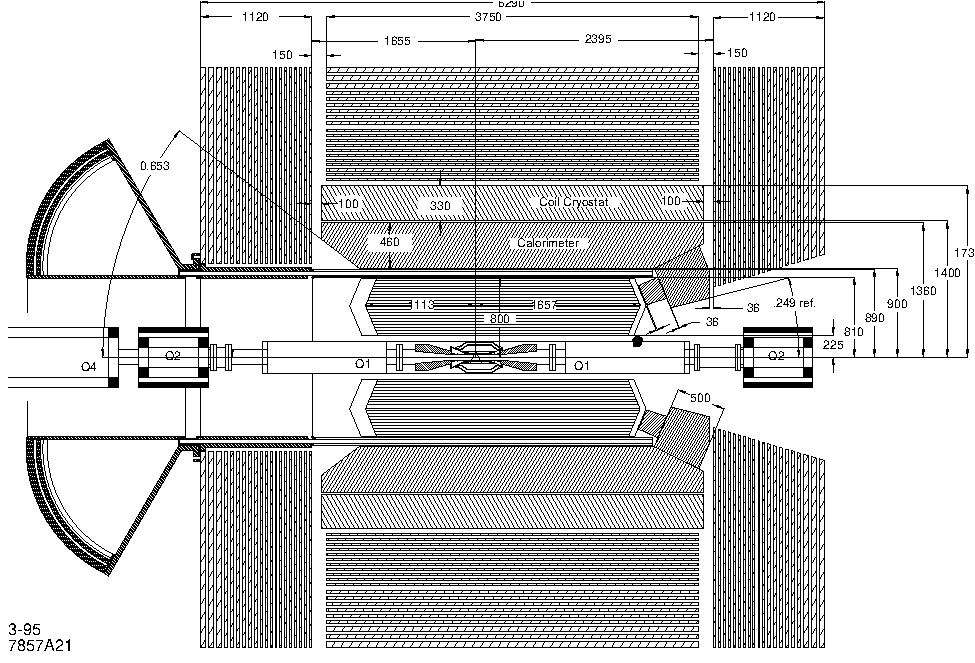
\includegraphics[width=0.7\textwidth]{figs/babar_detector_view.pdf}
    \caption{
        View of the \BaBar/ detector.
        Extracted from \cite{Boutigny:1995ib}.
    }
    \label{fig:babar_detector_view}
\end{figure}

% Talk about BaBar being 4 pi
In $e^- e^+$ detectors, $b \bar{b}$ is produced at all solid angles with
non-negligible probability \cite{Boutigny:1995ib,McGregor:2008ek}, thus the
detector needs to cover almost all solid angles (a $4\pi$ detector).
Indeed, \BaBar/ has tracking coverage of 0.92, namely 92\% of the $4\pi$ solid
angle.

% Talk about tracking and calorimeters
$B$ physics requires excellent vertex resolution and tracking, because the two
$B$ mesons produced by \Y4S/ must be reliably separated.
\BaBar/ has excellent tracking for charged particles, and sufficient spatial
and energy resolution in the electromagnetic calorimeter to reconstruct the
momenta of neutral particles \cite{Bauer:2005} with adequate precision.

%The LHC is a $pp$ collider, located at Geneva, Switzerland.
% Talk about the LHC being a hadron collider and the difficulties associated
% with it
Unlike electrons and positrons, the proton is a composite particle made of
$u, u, d$ quarks as well as other virtual partons.
All these particles participate in the $pp$ collision, carrying
varying portion of the total momentum.
The exact fraction of momentum carried by each type of parton is described by
parton distribution function\footnote{
    The parton distribution function is defined as:
    Number density to find fraction of the momentum (denoted as $x$) at certain
    squared energy scale $Q^2$.
} \cite{Ball:2014uwa}.
Since the precise fraction of momentum carried by interacting
partons\footnote{
    Again, these are characterized by parton distribution functions
} is unknown, the $B$ meson rest frame is not readily calculable.

Because many partons, such as quarks and gluons, can interact both
electroweakly and strongly,
the cross section of $b \bar{b}$ is larger than that of the $B$ factories, as a
result, more $b \bar{b}$ events are generated.
The measured $b \bar{b}$ cross section at LHCb in \SI{13}{TeV} $pp$
collisions\footnote{
    For $2 < \eta < 5$ only, since this is the LHCb acceptance range.
} is $144 \pm 1 \pm 21$~\si{\mu b} \cite{Aaij:2016avz}, whereas at the $B$
factories it is only about $1.05$~\si{nb} \cite{Harrison:1998yr}.
At the same time, unwanted particles will be generated frequently at hadron
colliders, leading to higher background.


% Talk about subdetectors
LHCb, a single-arm spectrometer, is one of the four large experiments at the
LHC.
Its constituent subdetectors, from closest to farthest from the collision point,
are shown in \autoref{fig:lhcb_detector_view}:
The Vertex Locator (VELO) provides precise measurements of track coordinates
close to the collision point.
Two Ring Imaging Cerencov counters (RICH1, RICH2) provide particle
identification for charged particles over a wide range of momentum.
The Tracker Turicensis (TT), Inner Tracker (IT), and Outer Tracker (OT) provide
additional tracking for charged particles and measure their momenta.
The calorimeters (ECAL and HCAL) have a first-level (L0) trigger to select
hadron, electron, and photon candidates based on their transverse momentum
$p_T$;
they also provide identification for the particles listed above;
finally, they provide energy and position measurements for these particles.
The Muon system (M1-5) is farthest from the collision point;
it provides L0 high $p_T$ muon trigger, and a high-level trigger (HLT) for muon
identification. Compared to the $B$ factories, LHCb has a much lower trigger
efficiency, which means many interesting events are filtered
out \cite{LHCb:2008}.

\begin{figure}[ht]
    \centering
    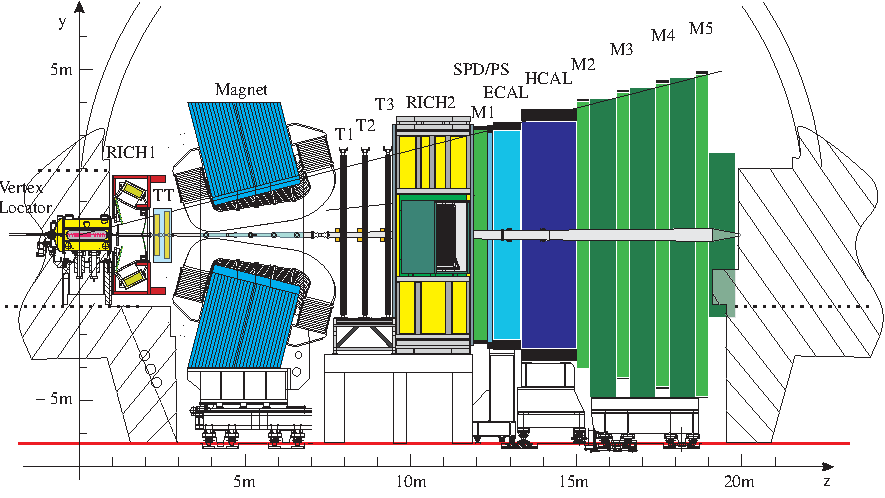
\includegraphics[width=0.7\textwidth]{figs/lhcb_detector_view.pdf}
    \caption{
        View of the LHCb detector and its subsystems.
        Extracted from \cite{LHCb:2003ab}.
    }
    \label{fig:lhcb_detector_view}
\end{figure}

% Talk about LHCb being forward-only
An interesting design choice is the geometry of the LHCb detector:
Instead of being a barrel $4\pi$ detector, it is forward-only.
This is because at high energies, $b\bar{b}$ is mostly produced in the forward
and backward direction.
The LHCb design is a very cost-effective way to construct a detector at the LHC
dedicated for $B$ physics.

% Talk about tracking
LHCb has a very good vertexing and tracking system, achieving vertex resolutions
down to 20~$\mu$m in a challenging environment.
However, due to the amount of material before the calorimeters and their poor
granularity,
reconstruction of neutral particles, such as $\pi_0$, is less
precise \cite{LHCb:2008,Guz:2017}.
This is why LHCb analyses typically focus on final states with charged particles
only, whereas $B$ factories can afford to use final states with neutral
particles.

% Talk about run 1 and run 2 luminosity
LHCb collected data from 2010 to 2012 with a center of mass energy of
\SI{8}{TeV}, and from 2015 to 2018 at \SI{13}{TeV}.
The total integrated luminosity during these two periods is about
\SI{9.2}{fb^{-1}} \cite{LHCb-Lumi:2019}.
% Talk about LS2 upgrade and LHCb's future
Currently, LHCb is shut down for an upgrade which will greatly increase the
readout rate of the detector starting in 2021.



\section{Review of previous measurements}

\subsection{2013 \BaBar/ $R(D^{(*)})$}
% 2015 BELLE (also hadronic tag)
% BELLE semileptonic tags

\subsection{2016 LHCb $R(D^{*})$}

\subsection{recent measurements from LHCb (forgot the decay channels)}
%2018 LHCb hadronic decay of Tau -> 3* Pi R(D*)


\section{Outlook for LHCb Run 2 $R(D^{(*)})$ measurements}
%\subsection{Current progress}

%\subsection{Expected improvements}

%\subsection{possible drawbacks}
% Remember: Run 2 supposedly has better pile-ups.

\PRLrule
\printbibliography
\end{document}